\section{Especificación de Requisitos}
En esta sección se establecen las necesidades y expectativas a cumplir, así como los elementos clave que guían el diseño y la implementación de la aplicación.

\subsection{Requisitos Funcionales}
La Tabla \ref{tabla:RF} recoge las funcionalidades específicas que el sistema debe ofrecer.

\begin{longtable}{ p{2.5cm} p{4cm} p{9cm}  }
    \caption{Requisitos  Funcionales} \label{tabla:RF} \\
    \hline
    \endfirsthead
    \multicolumn{3}{c}%
    {{\bfseries \tablename\ \thetable{}: Continuación de la tabla anterior}} \\
    \hline
    ID& Resumen& Descripción \\
    \hline
    \endhead
    
    \hline \multicolumn{3}{|r|}{{Continúa en la siguiente página}} \\ \hline
    \endfoot
    
    \hline
    \endlastfoot
    
    \textbf{RF-001}& Login y Registro & El sistema permitirá a los usuarios iniciar sesión con credenciales válidas o registrarse como nuevos 
    usuarios, proporcionando la funcionalidad básica de autenticación y creación de cuentas.\\
    \textbf{RF-002} & Edición completa del perfil por parte de los usuarios & Los usuarios dispondrán de la capacidad total para editar y
    actualizar la información de su perfil dentro del sistema, lo que incluirá datos personales y otros detalles relevantes, ofreciendo una 
    experiencia de usuario personalizada y adaptable.\\
    \textbf{RF-003} & Autorización de correo electrónico & Cuando un usuario se registre, se enviará un correo electrónico de verificación para 
    asegurar la autenticidad de la dirección de correo electrónico proporcionada.\\
    \textbf{RF-101} & Visualización de cantidad de usuarios registrados por mes & El administrador podrá ver la cantidad de usuarios que se han 
    registrado en el sistema durante cada mes.\\
    \textbf{RF-102} & Visualización de cantidad de usuarios por tipo & El administrador podrá ver la cantidad de usuarios registrados clasificados 
    por tipo (administrador, organizador, cliente) en el sistema.\\
    \textbf{RF-103} & Visualización de cantidad de eventos creados por mes & El administrador podrá ver la cantidad de eventos que se han creado en 
    el sistema durante cada mes.\\
    \textbf{RF-104} & Creación de usuarios de tipo Organización & Se dotará al administrador de la capacidad de crear usuarios con el rol específico 
    de 'Organización', lo que permitirá una gestión más detallada y especializada de usuarios dentro del sistema.\\
    \textbf{RF-105} & Filtrado de usuarios por tipo, nombre o email & Se integrará una función que permita al administrador obtener un 
    listado completo de todos los usuarios del sistema, con la posibilidad de aplicar filtros según su tipo de usuario, nombre o dirección 
    de correo electrónico para una búsqueda más eficiente y precisa.\\
    \textbf{RF-106} & Borrado de usuarios por parte del administrador & Se implementará la funcionalidad para que el administrador pueda 
    eliminar usuarios del sistema previa confirmación, permitiendo una gestión eficiente de la base de datos de usuarios y garantizando la integridad 
    y seguridad del sistema.\\
    \textbf{RF-107} & Obtener Usuario en el Sistema & Se implementará la funcionalidad para que el administrador pueda 
    ver información básicas de los usuarios registrados en el sistema\\
    \textbf{RF-108} & Borrado automático & Los usuarios que no hayan confirmado el correo en 15 minutos seran borrados automáticamente del sistema\\
    \textbf{RF-201} & Ver eventos creados por el organizador & El organizador tendrá la capacidad de ver los eventos que ha creado dentro del sistema.\\
    \textbf{RF-202} & Eliminación de eventos por el organizador & Se permitirá al organizador eliminar los eventos que ha creado dentro del sistema.\\
    \textbf{RF-203} & Edición de eventos por el organizador & El organizador podrá editar los eventos que ha creado, lo que incluirá la modificación de 
    detalles como nombre, descripción, fecha, etc.\\
    \textbf{RF-204} & Creación de eventos por el organizador & Se permitirá al organizador crear nuevos eventos proporcionando detalles como nombre, descripción, 
    fecha y, opcionalmente, contraseña para acceder al evento.\\
    \textbf{RF-205} & Visualización de cantidad de inscritos en eventos por el organizador & El organizador podrá ver la cantidad de usuarios inscritos en los 
    eventos que ha creado dentro del sistema.\\
    \textbf{RF-301} & Visualización de organizaciones por parte del cliente & Los clientes tendrán la capacidad de ver las organizaciones disponibles en el sistema.\\
    \textbf{RF-302} & Visualización de perfil de organizaciones por parte del cliente & Los clientes podrán ver el perfil de las organizaciones dentro del sistema.\\
    \textbf{RF-303} & Visualización de eventos de organizaciones por parte del cliente & Los clientes podrán ver los eventos que ofrecen las organizaciones dentro del sistema.\\
    \textbf{RF-304} & Inscripción a eventos por parte del cliente & Los clientes podrán inscribirse a los eventos ofrecidos por las organizaciones dentro del sistema.\\
    \textbf{RF-305} & Eventos privados con contraseña & Se permitirá la creación de eventos privados que requieran una contraseña para acceder a ellos.\\
    \textbf{RF-306} & Generación de entradas para eventos & Una vez adquirida la entrada, se generará un código QR para acceder al evento.\\
    \textbf{RF-307} & Manejo de Concurrencia \ref{sec:concurrencia} & En caso de que dos usuarios intenten adquirir una entrada simultáneamente, se debe implementar 
    un sistema de colas para evitar incongruencias en la base de datos. \\
    \textbf{RF-308} & Descarga de PDF de la Entrada & Los Clientes tienen que tener la opción de poder descargar la entrada en formato PDF para poder
    compartirla si quisieran\\
    \end{longtable}
    \newpage
    \subsection{Requisitos No Funcionales}
    La Tabla \ref{tabla:RNF} recoge las funcionalidades para mejorar la experiencia del usuario, se abordan tanto las limitaciones 
    técnicas como los factores a considerar.

    \begin{longtable}{ p{2.5cm} p{4cm} p{9cm} }
        \caption{Requisitos No Funcionales} \label{tabla:RNF} \\
        \hline
        ID & Resumen & Descripción \\
        \hline
        \endfirsthead
        \multicolumn{3}{c}{{\bfseries \tablename\ \thetable{}: Continuación de la tabla anterior}} \\
        \hline
        ID & Resumen & Descripción \\
        \hline
        \endhead
        \hline \multicolumn{3}{|r|}{{Continúa en la siguiente página}} \\ \hline
        \endfoot
        \hline
        \endlastfoot
        \textbf{RNF-001} & Desempeño del sistema & El sistema debe ser capaz de manejar hasta 1000 usuarios simultáneos sin experimentar una degradación 
        significativa del rendimiento. \\
        \textbf{RNF-002} & Seguridad de los datos & Todos los datos sensibles almacenados en el sistema deben estar cifrados utilizando un algoritmo de cifrado 
        estándar. \\
        \textbf{RNF-003} & Usabilidad & La interfaz de usuario debe ser intuitiva y fácil de usar, con tiempos de carga de página inferiores a 1 segundo para 
        mejorar la experiencia del usuario. \\
        \textbf{RNF-004} &  Conexión a Internet & El sistema debe tener acceso a Internet para permitir la comunicación con servicios externos y el intercambio
         de datos. \\
        \textbf{RNF-005} & Rendimiento & El sistema debe responder a las solicitudes del usuario dentro de un tiempo aceptable, con tiempos de carga de página y
         operaciones de procesamiento mínimos. \\
        \textbf{RNF-006} & Accesibilidad & Tiene que ser posible usar la aplicación de forma óptima en dispositivos móviles\\ 
    \end{longtable}

\section{Arquitectura y análisis}

\textbf{Enterprise Event Solutions} es una aplicación \textbf{Fullstack} creada siguiendo un patrón de diseño MVC. A continuación, se muestra un plano general
que será desglosado:

\subsection{Arquitectura general}
Cada uno de los componentes definidos en la Figura \ref{fig:mvc_architecture} representa a nivel general los componentes que forman EVS: backend, frontend y base de dato, todas
estas dockerizadas y desplegadas en un servicio de AWS EC2 y utilizando Elastic IP para asignar una IP pública fija.

\begin{figure}[h]
    \centering
    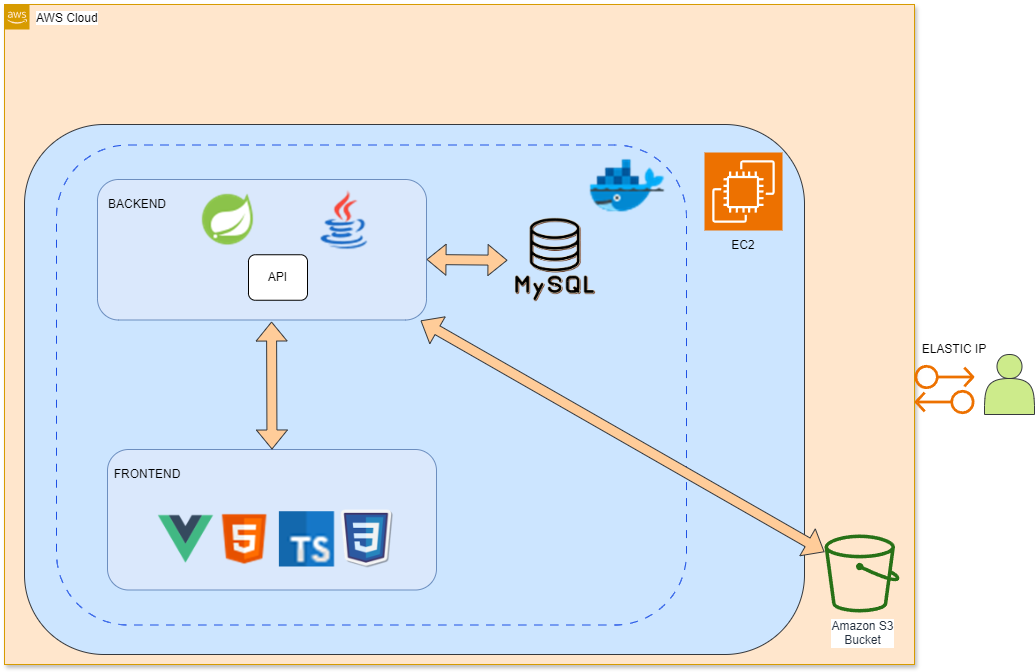
\includegraphics[width=0.9\textwidth]{Aquitectura1.png} 
    \caption{Diagrama de Arquitectura de EVS}
    \label{fig:mvc_architecture}
\end{figure}

La figura \ref{fig:mvc_architecture} muestra el diagrama de arquitectura de EVS desplegado en la nube de AWS. La arquitectura está dividida en dos componentes principales: el backend y el frontend.

El backend utiliza Spring Boot (Java) para la lógica de negocio y se conecta a una base de datos MySQL. La base de datos está contenedorizada con Docker y se ejecuta en una
instancia EC2 de AWS. La API del backend se comunica con el frontend y con la base de datos MySQL.

El frontend está desarrollado con tecnologías web: Vue.js, HTML5, TypeScript y CSS3 son las más relevantes. Los usuarios acceden a la aplicación a través de una dirección 
IP elástica asignada a la instancia EC2.

Además, el almacenamiento de archivos se maneja utilizando un bucket de Amazon S3, que interactúa con el backend para gestionar los archivos de la aplicación.

En resumen, esta arquitectura de EVS en AWS muestra una solución escalable y eficiente, utilizando tecnologías modernas para el desarrollo web y servicios en la nube para el despliegue y almacenamiento. 
\textbf{Enterprise Event Solutions} combina las fortalezas de \textbf{SpringBoot} y \textbf{Vue.js} en un patrón MVC para ofrecer una solución robusta y 
escalable. Con el soporte de \textbf{AWS} y \textbf{MySQL}, la aplicación está preparada para manejar grandes volúmenes de datos y ofrecer una experiencia 
de usuario fluida.

\newpage
\section{Flujo de la Aplicación}

En esta sección se presenta el diagrama de flujo de la aplicación dividida en partes para su mejor comprensión.
\begin{figure}[h]
    \centering
    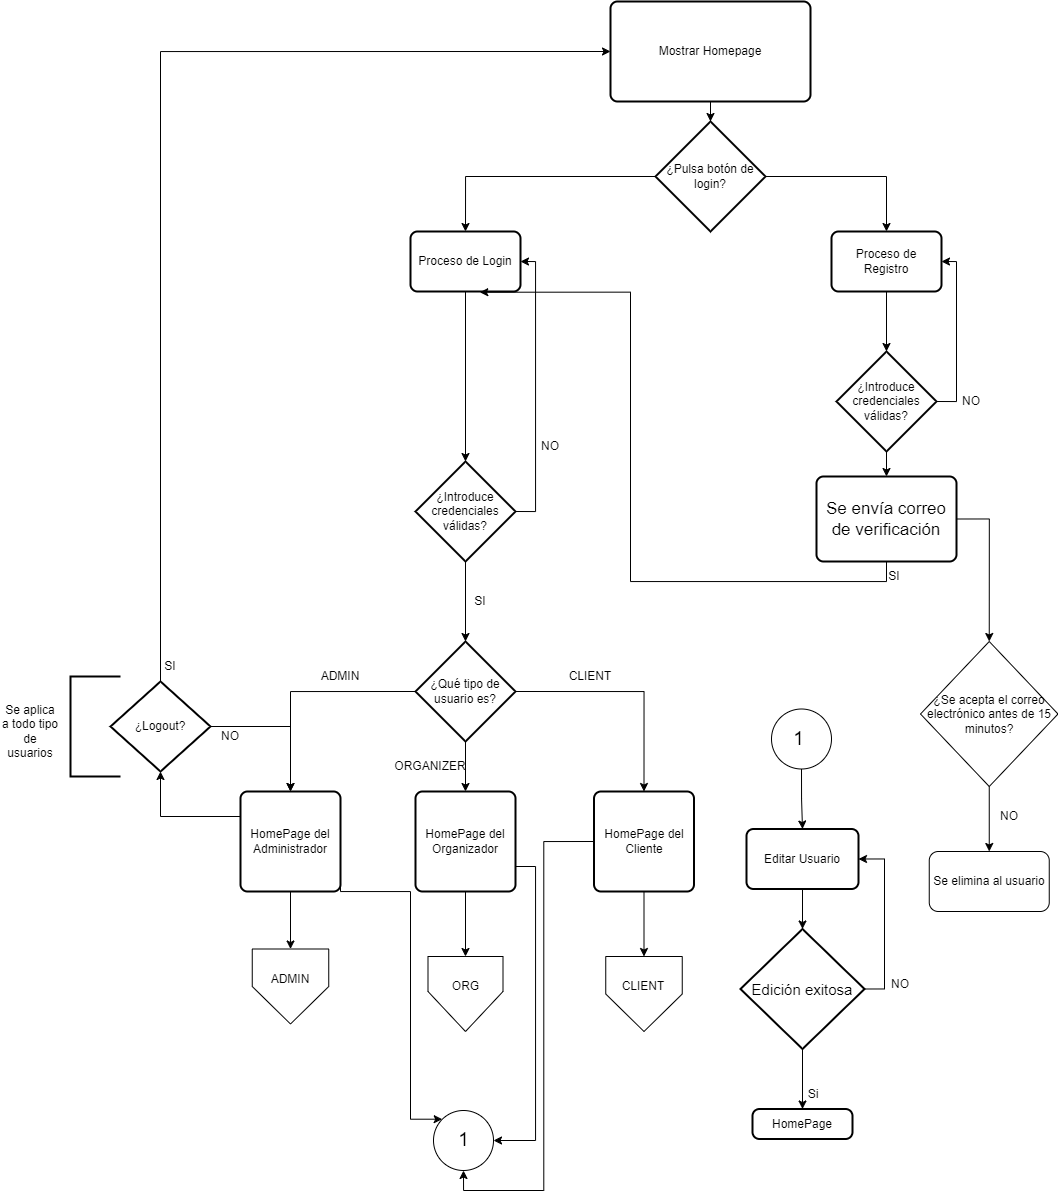
\includegraphics[width=0.9\textwidth]{FlujoGeneral.png} 
    \caption{Diagrama de Flujo Parte 1}
    \label{fig:flujoEvs}
\end{figure}
\newpage
\begin{figure}[h]
    \centering
    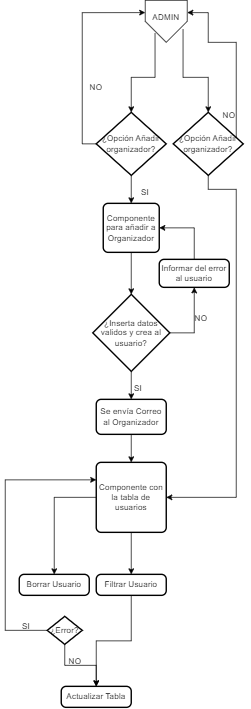
\includegraphics[width=0.4\textwidth]{AdminFlujo.png} 
    \caption{Diagrama de Flujo Parte 2}
    \label{fig:flujoEvs1}
\end{figure}
\newpage
\begin{figure}[h]
    \centering
    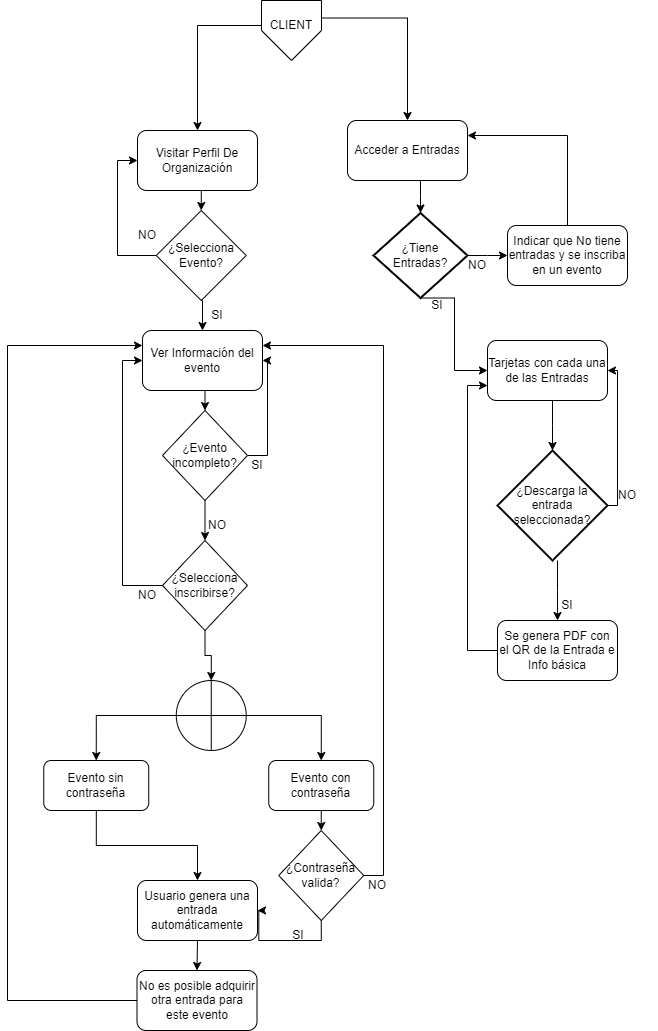
\includegraphics[width=0.7\textwidth]{Cliente.png} 
    \caption{Diagrama de Flujo Parte 3}
    \label{fig:flujoEvs2}
\end{figure}
\newpage
\begin{figure}[h]
    \centering
    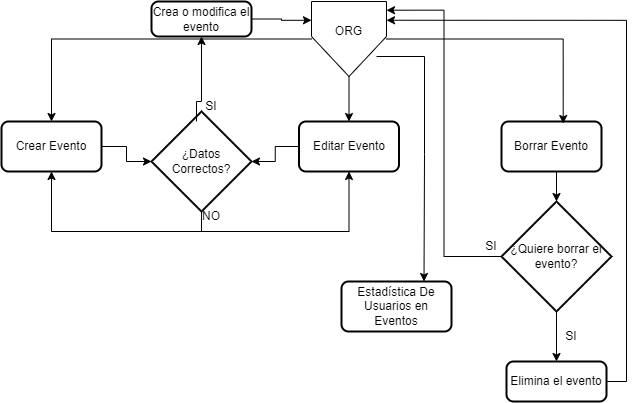
\includegraphics[width=0.8\textwidth]{Org.png} 
    \caption{Diagrama de Flujo Parte 4}
    \label{fig:flujoEvs3}
\end{figure}
\section{Diseño e implementación}    
\subsection{Modelo}
La persistencia en Enterprise Event Solutions se sustenta en una serie de Entidades almacenadas en una base de datos con la que los servicios interactuan mediante
las interfaces proporcionadas por JPA \ref{sec:jpa}. Es el pilar fundamental en el que se sustenta el modelo de negocio de la aplicación.
\begin{figure}[h]
    \centering
    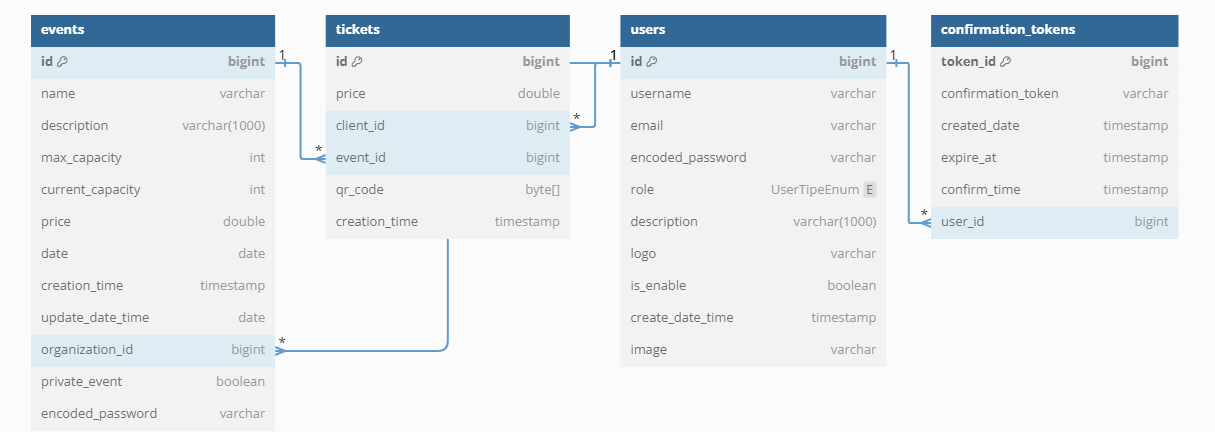
\includegraphics[width=1.0\textwidth]{EVSdiagra.png} 
    \caption{Modelo E-R de la BD}
    \label{fig:diagramaBD}
\end{figure}

\subsubsection{JPA}
\label{sec:jpa}

JPA (Java Persistence API) es una especificación de Java que facilita la gestión de la persistencia de datos en aplicaciones Java.
En Spring, se usa para simplificar las operaciones CRUD y el manejo de relaciones entre entidades, permitiendo trabajar con objetos en lugar de SQL. 
Spring Data JPA integra JPA en el ecosistema Spring, proporcionando repositorios predefinidos para operaciones de base de datos comunes.

A continuación se muestra un fragmento de código de Spring Data JPA en Java:
\myjavastyle
\begin{lstlisting}[language=Java, caption=Ejemplo de Repositorio en Spring Data JPA, label=lst:jpacodigo]
@Repository
public interface UserRepository extends JpaRepository<User,Long> {
    public Optional<User> findByEmail(String email);
    public List<User> findAllByRole(UserTipeEnum type);
    public Optional<User> findByUsername(String username);
}
\end{lstlisting}

Como se puede observar, gracias a la gran potencia de Spring y de JPA, simplemente con crear una interfaz con métodos que creemos que vamos a necesitar en 
nuestros servicios, y sin la necesidad de añadir @Querys, podemos hacer consultas sobre la base de datos.

Pero también podemos hacer nuestras propias Querys sobre la base de datos:
\myjavastyle
\begin{lstlisting}[language=Java, caption=Ejemplo de Query  en Spring Data JPA]
    @Query("SELECT u FROM _user u WHERE u.isEnable = false AND u.createDateTime < :fifteenMinutesAgo")
    List<User> findByEnableFalseAndCreateDateTimeBefore(LocalDateTime fifteenMinutesAgo);
\end{lstlisting}

\subsection{Controlador}
La creación de controladores me ha permitido gestionar un sistema de endpoints que sirve como la interfaz principal 
para la comunicación entre el cliente y el servidor. Estos controladores se encargan de recibir las solicitudes HTTPS de delegar el procesamiento a 
los servicios correspondientes. Los servicios encapsulan la lógica de negocio y se comunican con los repositorios JPA para acceder a los datos de la 
base de datos de manera eficiente. Además, para garantizar la seguridad, se utiliza JWT (JSON Web Tokens), que permite la autenticación y autorización 
de los usuarios. Los tokens JWT se generan tras un inicio de sesión exitoso y se utilizan para proteger los endpoints, asegurando que solo los usuarios 
autenticados puedan acceder a recursos específicos. Este enfoque no solo organiza el código de manera modular y mantenible, sino que también proporciona 
una robusta capa de seguridad para la API.

En la figura \ref{fig:class_architecture} se puede observar un desglose de las clases del backend y las interrelaciones.

\begin{figure}[h]
    \centering
    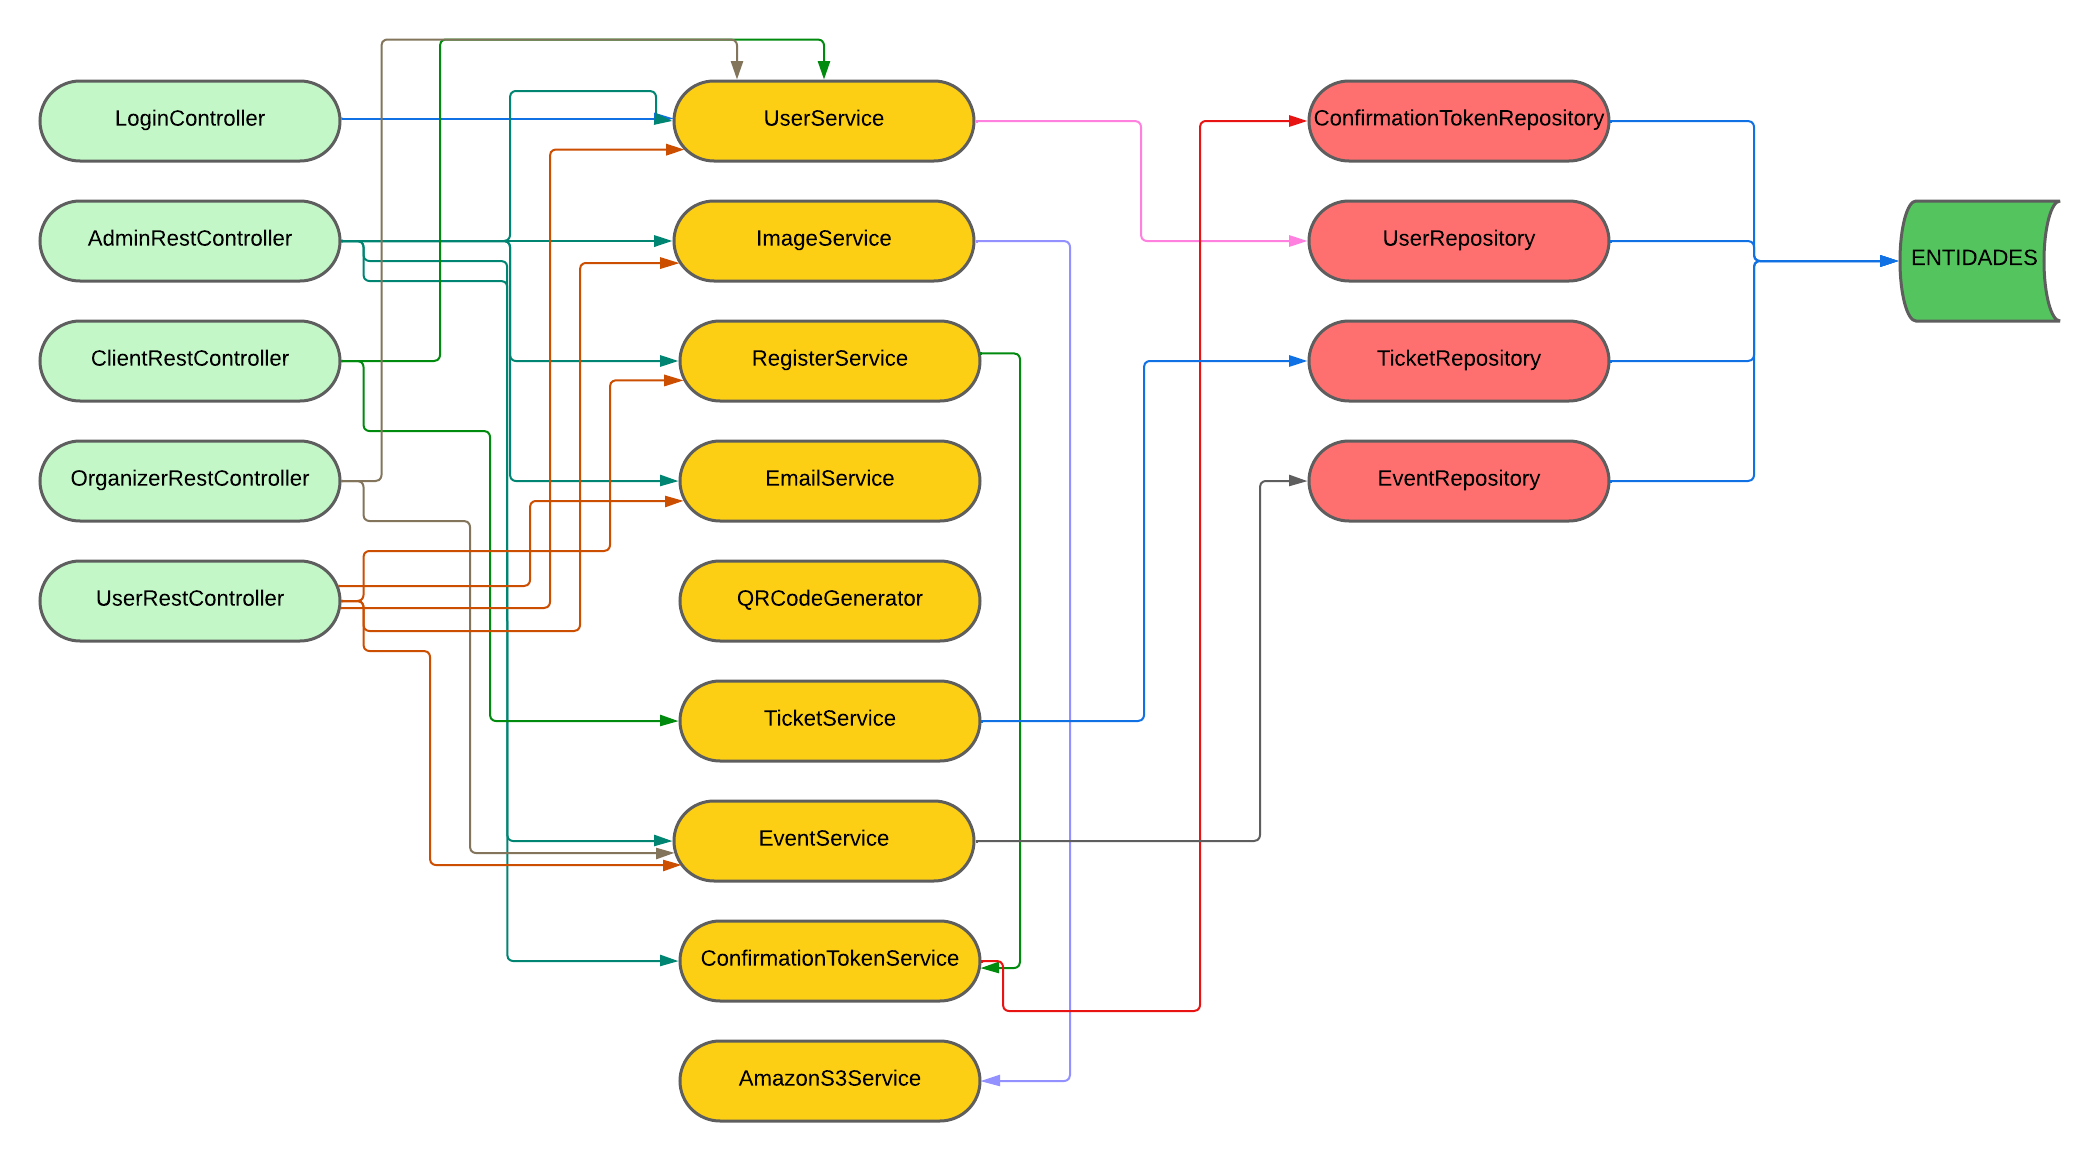
\includegraphics[width=1\textwidth]{DiagramaClases.png} 
    \caption{Diagrama de Clases de EVS}
    \label{fig:class_architecture}
\end{figure}

Además he implementado otras configuraciones para añadir una capa extra de seguridad a la aplicación como configuración CSRF y CORS para limitar las url 
que pueden hacer uso de los endpoints de la app. Por supuesto se han creado las configuraciones necesarias para manejar las tecnologías externas como S3, dentro de 
EVS.

\begin{figure}[h]
    \centering
    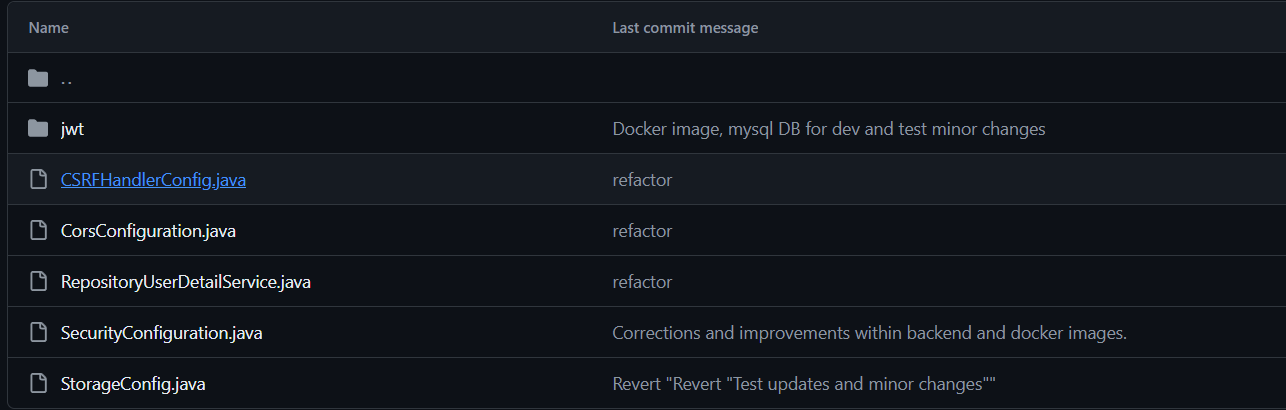
\includegraphics[width=1\textwidth]{security.png} 
    \caption{Seguridad del backend}
    \label{fig:securityClasses}
\end{figure}

Durante la fase de desarrollo se hizo uso de Postman para realizar consultas a la API y verificar el correcto funcionamiento de esta. Además se generó la documentación de la
misma con Swagger y en el repositorio de GitHub se encuentra tanto una Colección de Postman para hacer uso de esta API como la documentación de esta en formato JSON.

\begin{figure}[h]
    \centering
    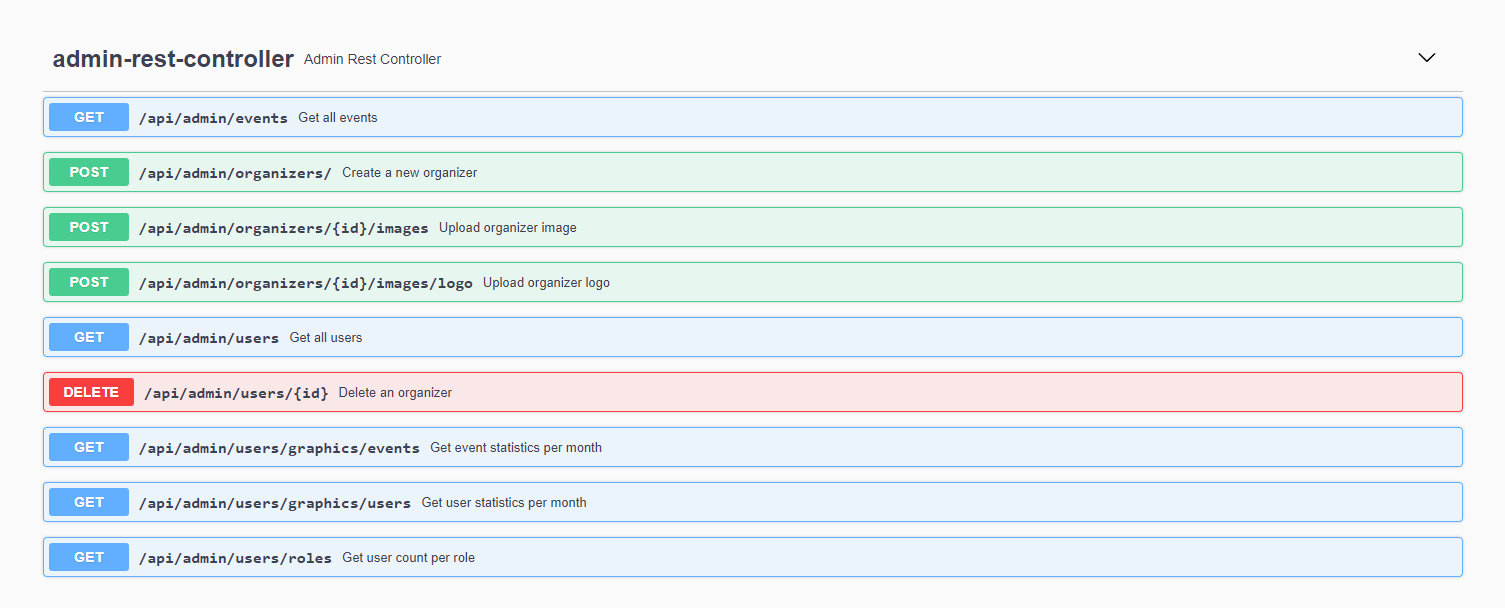
\includegraphics[width=1\textwidth]{Swagger1.png} 
    \caption{Documentación Swagger 1}
    \label{fig:swagger}
\end{figure}
\newpage
\begin{figure}[h]
    \centering
    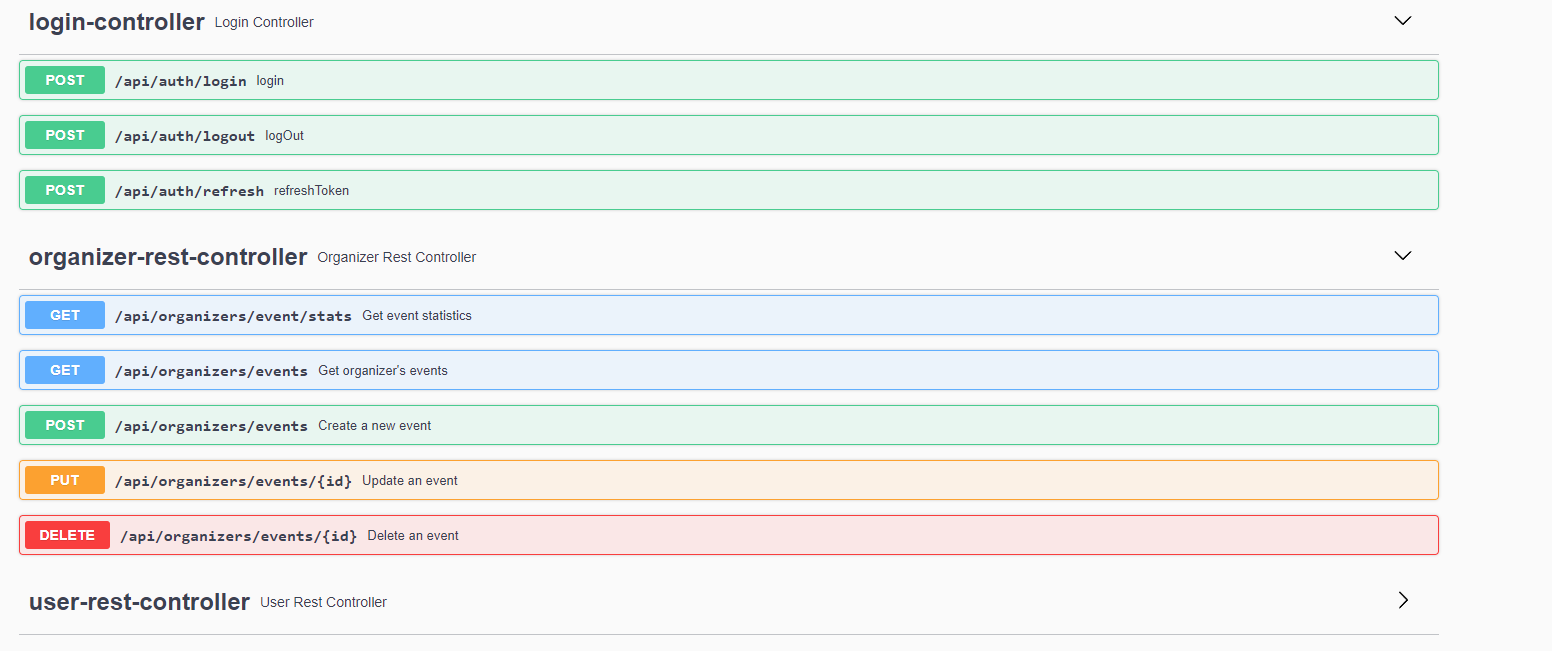
\includegraphics[width=1\textwidth]{Swagger2.png} 
    \caption{Documentación Swagger 2}
    \label{fig:swagger2}
\end{figure}

\subsection{Vista}
El frontend de Enterprise Event Solutions ha sido implementado en Vue.js. Específicamente en Vue3, que trae consigo algunos cambios con respecto a su versión
anterior Vue2. La utilización de este framework me ha permitido añadir tanto bibliotecas de componentes y gráficos (Bootstrap5 y Chart.js respectivamente)
como relaciones entre los diferentes componentes basado en "props", permitiendo de esta manera diferentes comportamientos del componente dependiendo de
que valores se le pasen en el componente padre.

Un ejemplo del uso de estas props sería:
\myvuestyle
\begin{lstlisting}[language=HTML, caption=Ejemplo del Padre, label=lst:padre]
    <event_cards
    :evento="evento"
    :is-org="false"
    >
    </event_cards>
\end{lstlisting}
\myvuestyle
\begin{lstlisting}[language=HTML, caption=Ejemplo del Hijo, label=lst:hijo]
    <script lang="ts">
    import {EventService} from "../services/event.service";
    import { useRouter } from "vue-router";
    import { Event } from "../models/Event";
    import { computed, ref } from "vue";
    export  default {
        name: "event_cards",
        props:{
          evento: Object as ()=> Event,
          isOrg: Boolean,
        },
    }
\end{lstlisting}

En el código \ref{lst:padre}, se observa que se inserta en el template un componente con la información del evento. Por otro lado, en el código 
\ref{lst:hijo}, se manejan estos valores que hemos pasado desde el componente padre. En este fragmento, si se le pasa \texttt{true} en la variable 
\texttt{is-org}, el componente tendrá un comportamiento diferente a si se le pasa \texttt{false}. Ademas en la variable \texttt{evento} le pasamos la información
del evento para garantizar la reactividad de los componentes de forma individual. De esta forma trabajamos con módulos y no con un elemento.

\newpage
En las figuras \ref{fig:eventosCli} y \ref{fig:orgMain}  se puede ver el mismo componente con Props diferentes.
\begin{figure}[h]
    \centering
    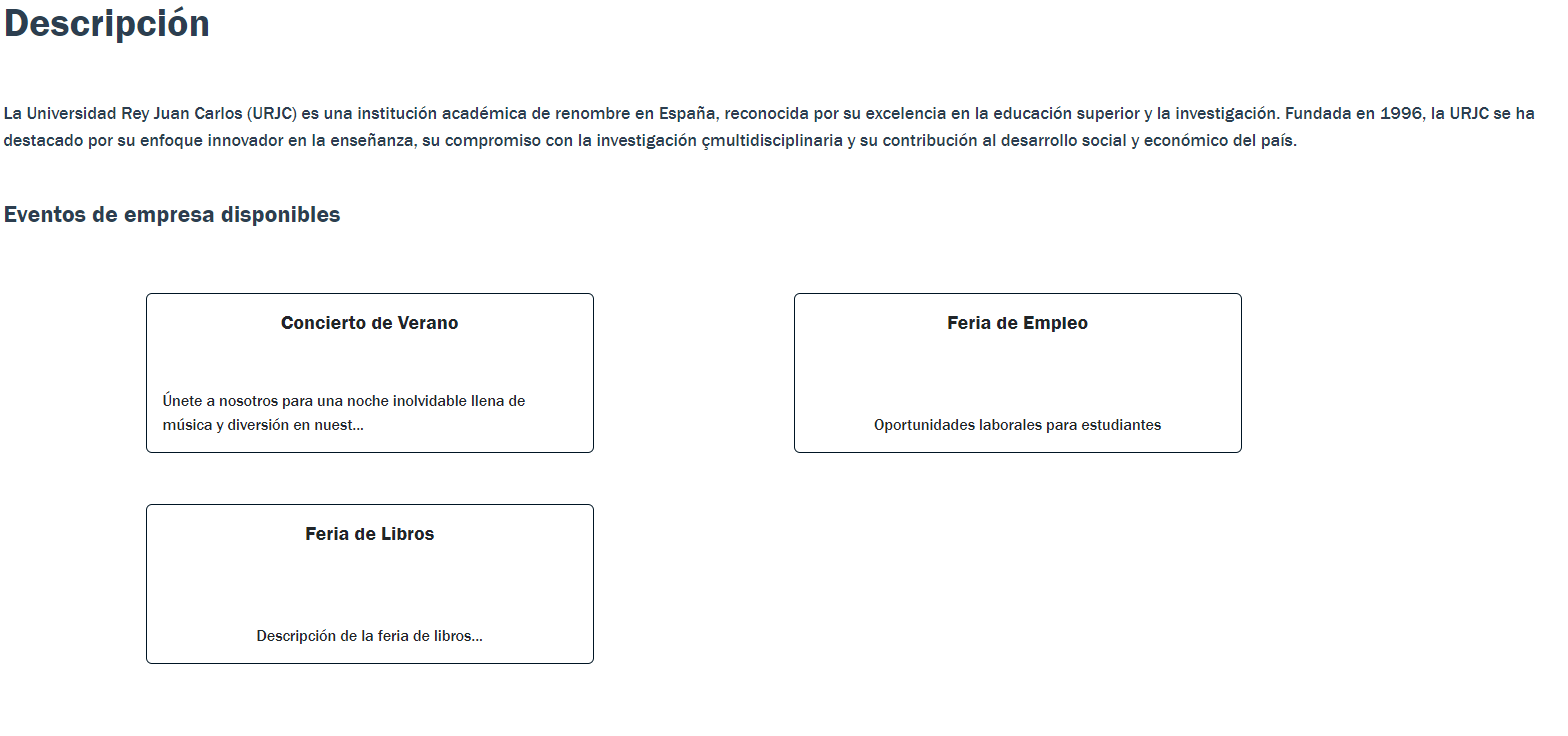
\includegraphics[width=1\textwidth]{eventosCli.png} 
    \caption{Componente Eventos para el Cliente}
    \label{fig:eventosCli}
\end{figure}

\begin{figure}[h]
    \centering
    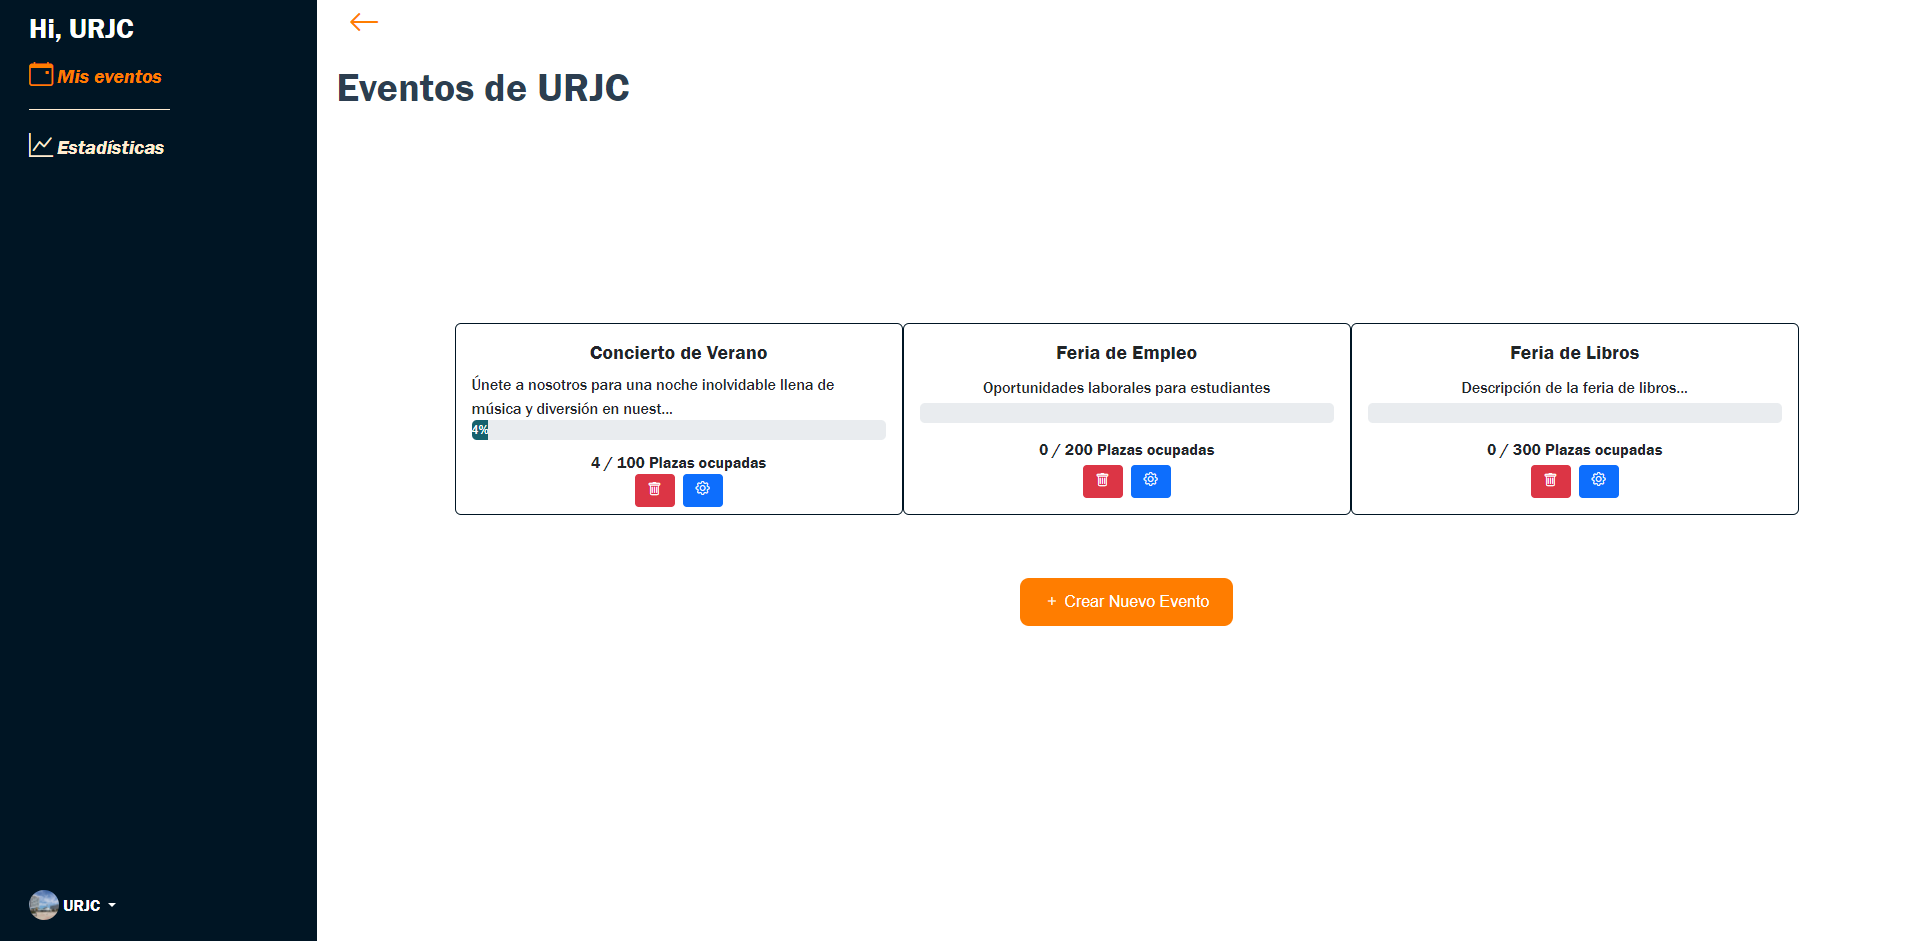
\includegraphics[width=1\textwidth]{orgMain.png} 
    \caption{Componente Eventos para el Organizador}
    \label{fig:orgMain}
\end{figure}


\subsection{Concurrencia en los eventos}
\label{sec:concurrencia}
La problemática de la adquisición de entradas para eventos con capacidad limitada se presenta cuando una gran cantidad de personas intenta acceder simultáneamente
para comprar entradas. Este fenómeno, común en eventos populares, puede causar varios problemas, entre ellos:
\begin{itemize}
    \item Sobreventa de Entradas: Cuando múltiples usuarios intentan comprar entradas al mismo tiempo, existe el riesgo de que el sistema venda más entradas de las disponibles.
    Esto ocurre debido a la falta de sincronización adecuada entre las solicitudes concurrentes, lo que puede llevar a la creación de la misma entrada a múltiples usuarios.
    \item Condiciones de Carrera: Las condiciones de carrera suceden cuando dos o más procesos acceden a recursos compartidos (en este caso, la base de datos de entradas) al mismo
    tiempo y los resultados dependen del orden en que se ejecutan. Esto puede provocar inconsistencias en los datos y errores en la asignación de entradas.
    \item Experiencia del Usuario: Un sistema que no maneja adecuadamente la concurrencia puede llevar a tiempos de respuesta lentos, errores y una experiencia de usuario
    insatisfactoria. Los usuarios pueden experimentar frustración si el sistema falla repetidamente o si no están seguros de si su adquisición ha sido exitosa.   
\end{itemize}

Para abordar estos problemas, se ha utilizado la anotación @Transactional de JPA. Esta solución implica:
\begin{itemize}
    \item Aislamiento de Transacciones: La anotación @Transactional asegura que cada operación de compra de entradas se ejecute en una transacción aislada. Esto significa
    que los cambios realizados por una transacción no serán visibles para otras transacciones hasta que se complete. Esto ayuda a prevenir la sobreventa de entradas
    al garantizar que cada transacción compruebe y reserve las entradas de manera exclusiva.
    \item Gestión Automática de Transacciones: Con @Transactional, la gestión de transacciones se maneja automáticamente, simplificando el desarrollo y reduciendo la posibilidad
    de errores humanos. Si una transacción falla, se realiza un rollback automático, asegurando que la base de datos se mantenga en un estado consistente.
    \item Control de Concurrencia: JPA proporciona varios niveles de aislamiento de transacciones que pueden ser utilizados para controlar la concurrencia. Estos niveles determinan
    cómo y cuándo los cambios realizados por una transacción se vuelven visibles para otras transacciones, ayudando a evitar las condiciones de carrera.
\end{itemize}

En resumen, la utilización de @Transactional en JPA permite manejar de manera efectiva la concurrencia durante la adquisición de entradas para eventos. Esta estrategia
asegura que cada transacción de adquisición de entradas se procese de forma segura y aislada, manteniendo la integridad de los datos y proporcionando una mejor experiencia de
usuario.

\subsubsection{Desarrollo de la función}
En este apartado se explicará de menor a mayor nivel la implementación de esta funcionalidad y finalmente se explicará el test desarrollado para probarla.

\subsubsection*{Repositorio}
El código \ref{lst:jpaconcurrente} actualiza la capacidad actual de un evento específico, incrementándola en 1 si no se excede la capacidad máxima permitida. 
Utiliza una consulta JPQL definida con @Query para actualizar el campo current\_capacity, bajo la condición de que la nueva capacidad no supere max\_capacity. 
La consulta se aplica al evento con el ID proporcionado como parámetro. El método devuelve un entero indicando el éxito o el fracaso de la operación. Esto es crucial para
prevenir la sobreventa y mantener la consistencia de los datos durante la adquisición de entradas.

\myjavastyle
\begin{lstlisting}[language=Java, caption=Función incrementCurrentCapacity, label=lst:jpaconcurrente]
    @Transactional
    @Modifying
    @Query("UPDATE Event e SET e.current_capacity = e.current_capacity + 1 WHERE e.id = :id AND e.current_capacity + 1  <= e.max_capacity")
    public int incrementCurrentCapacity(@Param("id") Long id);
\end{lstlisting}

\subsubsection*{Servicios}
En primer lugar, se hace uso de esta función en el servicio EventService. En el código se verifica si un evento específico está lleno al intentar incrementar su capacidad 
actual en uno. Primero, verifica la existencia del evento por su ID utilizando eventExists(id). Luego, intenta incrementar la capacidad actual del evento mediante 
eventRepository.incrementCurrentCapacity(id). Si la operación tiene éxito (devolviendo 1), devuelve el evento; de lo contrario, lanza una excepción indicando que el 
evento está lleno. Este proceso garantiza la integridad de la transacción al manejar concurrencia y prevenir la sobreventa durante la gestión de entradas para eventos.
\myjavastyle
\begin{lstlisting}[language=Java, caption=Función incrementCurrentCapacity, label=lst:servicioEvento] 
    public Event checkIfFull(long id){
        Event event = eventExists(id);

        int i = eventRepository.incrementCurrentCapacity(id);
        if(i==1){
            return event;
        }else{
            throw new ResponseStatusException(HttpStatus.CONFLICT,"This event is full");
        }
    }

    public void deleteEvent(Event event){
        eventRepository.delete(event);
    }

    private Event eventExists(Long eventId){
        Optional<Event> opEvent = eventRepository.findById(eventId);
        if (opEvent.isEmpty()) {
            throw new ResponseStatusException(HttpStatus.BAD_REQUEST, "Event not longer exist");
        }
        return opEvent.get();
    }
\end{lstlisting}
En segundo lugar se hace uso de este método en TicketService, donde verdaderamente se adquirirá la entrada para el evento seleccionado. El código \ref{lst:servicioTicket} se encarga de crear un ticket
para un usuario en un evento, gestionando dos casos según la privacidad del evento y verificando la capacidad antes de emitir el ticket. Primero, se obtiene el evento y se
verifica si está lleno. Si el evento no es privado, se crea el ticket directamente. Si es privado, se verifica la contraseña antes de crear el ticket. Se genera un código QR
con los detalles del evento y se guarda el ticket en la base de datos, asegurando la integridad de la transacción y evitando la sobreventa durante la emisión de tickets.
\myjavastyle
\begin{lstlisting}[language=Java, caption=Función createTicket, label=lst:servicioTicket]
    public Ticket createTicket(User user,Long id,String passwordToCheck) throws IOException, WriterException {
        SimpleDateFormat dateFormat = new SimpleDateFormat("dd-MM-yyyy HH:mm");
        Event event = eventService.findById(id).orElseThrow();

        if (!event.isPrivateEvent()){
            eventService.checkIfFull(id);

            Ticket ticket = new Ticket(user,event);
            ticket.setPrice(event.getPrice());
            String formattedDate = dateFormat.format(event.getDate());
            saveTicket(ticket);
            String qrCodeData = "Identificador: " + ticket.getId() + ", Nombre del Evento: " + event.getName() + ", Fecha del evento: "+ formattedDate;
            byte[] qrCodeBytes = qrCodeGenerator.generateQRCode(qrCodeData, 200, 200);
            ticket.setQrCode(qrCodeBytes);
            saveTicket(ticket);

        return ticket ;
        }else{
         if (checkPassword(event.getEncodedPassword(),passwordToCheck)){
             eventService.checkIfFull(id);
             Ticket ticket = new Ticket(user,event);
             ticket.setPrice(event.getPrice());
             String formattedDate = dateFormat.format(event.getDate());
             saveTicket(ticket);
             String qrCodeData = "Identificador: " + ticket.getId() + ", Nombre del Evento: " + event.getName() + ", Fecha del evento: "+ formattedDate;
             byte[] qrCodeBytes = qrCodeGenerator.generateQRCode(qrCodeData, 200, 200); // Ajusta el tamaño del QR según tus necesidades
             ticket.setQrCode(qrCodeBytes);
             saveTicket(ticket);
             return ticket ;
         }
         else
             {return null;}
        }
    }
\end{lstlisting}

\subsubsection{Controlador}
Finalmente la clase ClientRestController, en concreto el método "buyTicket", como se muestra en el código \ref{lst:controladorClient}, se implementa un endpoint POST en un controlador de Spring MVC
para comprar un ticket. Utiliza la información del usuario autenticado para buscar su perfil completo. Luego, intenta crear un ticket para un evento especificado, utilizando
una contraseña opcional para eventos privados. Si la operación tiene éxito, devuelve el ticket con un estado HTTP 201 Created. Si hay un problema durante la creación del
ticket, responde con HTTP 503 Service Unavailable. Si la contraseña para un evento privado no es válida, devuelve HTTP 401 Unauthorized.
\myjavastyle
\begin{lstlisting}[language=Java, caption=Función buyTicket, label=lst:controladorClient]
    @PostMapping("/tickets/")
    public ResponseEntity<Ticket> buyTicket(HttpServletRequest request, @RequestParam Long id, @RequestBody(required = false) String password) {
        Principal principal = request.getUserPrincipal();
        User user = userService.findByEmail(principal.getName()).orElseThrow();
        String passwordSent;
        try {
            passwordSent = (password == null) ? "" : password;
            Ticket ticket = ticketService.createTicket(user, id, passwordSent);
            if (ticket != null)
                return new ResponseEntity<>(ticket, HttpStatus.CREATED);
        } catch (Exception e) {
            return new ResponseEntity<>(HttpStatus.SERVICE_UNAVAILABLE);
        }
        return new ResponseEntity<>(HttpStatus.UNAUTHORIZED);
    }
\end{lstlisting}

\subsubsection{Test asociado}
Como se esperaba, se ha realizado una prueba que verifique el correcto funcionamiento de la gestión de la concurrencia en la adquisición de entradas. 

El código \ref{lst:testConcurrencia} prueba concurrentemente la compra de tickets para un evento usando múltiples hilos. Primero, se crea un evento de prueba con una capacidad máxima y organizador
específicos, guardado mediante eventService.saveEvent(testEvent). Se configura un número elevado de hilos (numberOfThreads) para simular solicitudes concurrentes de compra
de tickets. Cada hilo crea un usuario único y realiza una solicitud HTTP simulada usando mockMvc.perform, que intenta comprar un ticket para el evento especificado.

Se utiliza CountDownLatch para coordinar la ejecución simultánea de los hilos: latch para sincronizar el inicio de todos los hilos y doneLatch para esperar a que todos los
hilos terminen. Cada hilo verifica el resultado de la solicitud HTTP esperando un código de estado HTTP 201 Created si la compra fue exitosa, o HTTP 409 Conflict si el evento
está lleno. Finalmente, se verifica que la capacidad actual del evento se ajuste correctamente al máximo después de todas las operaciones concurrentes.

\myjavastyle
\begin{lstlisting}[language=Java, caption=Función buyTicket, label=lst:testConcurrencia]
@DisplayName("Concurrent Ticket Purchase Test")
@ParameterizedTest(name = "{index} {0}")
@ValueSource(strings = {"client@urjc.es"})
public void concurrentTicketPurchaseTest(String username) throws Exception {
    Event testEvent = new Event();
    testEvent.setName("Test Event");
    testEvent.setMax_capacity(10);
    testEvent.setCurrent_capacity(0);
    Calendar calendar = Calendar.getInstance();
    calendar.set(2025, Calendar.AUGUST, 5, 18, 30);
    testEvent.setDate(calendar.getTime());
    testEvent.setOrganization(organizer);
    eventService.saveEvent(testEvent);

    int numberOfThreads = 15; // More than max capacity to test concurrency issues
    CountDownLatch latch = new CountDownLatch(1);
    CountDownLatch doneLatch = new CountDownLatch(numberOfThreads);

    ExecutorService executorService = Executors.newFixedThreadPool(numberOfThreads);

    for (int i = 0; i < numberOfThreads; i++) {
    int userIndex = i; // Final variable to use inside the lambda
    executorService.execute(() -> {
    try {
        // Creating a unique client user for each thread
        String uniqueUsername = username + userIndex;
        User client = new User("Client", uniqueUsername, "pass");
        userService.saveUser(client);

        System.out.println("User created: " + uniqueUsername);

        latch.await(); // wait for the starting signal

        mockMvc.perform(post("/api/clients/tickets/?id=" + testEvent.getId())
            .with(SecurityMockMvcRequestPostProcessors.user(client.getEmail()).password("pass"))) // Simulating authenticated user
            .andExpect(result -> {
                int status = result.getResponse().getStatus();
                if (status == HttpStatus.SC_CONFLICT) {
                    assertThat(status).isEqualTo(HttpStatus.SC_CONFLICT);
                } else {
                    assertThat(status).isEqualTo(HttpStatus.SC_CREATED);
                }
            })
            .andDo(print());
    } catch (Exception e) {
        e.printStackTrace();
        System.out.println("Error in thread: " + userIndex + " with message: " + e.getMessage());
    } finally {
        doneLatch.countDown();
    }
});
}

latch.countDown(); // Start all threads
doneLatch.await(); // Wait for all threads to finish

// Verify the number of tickets created
Event updatedEvent = eventService.findById(testEvent.getId()).orElseThrow();
assertThat(updatedEvent.getCurrent_capacity()).isEqualTo(testEvent.getMax_capacity());

executorService.shutdown();
}
\end{lstlisting}



\subsection{Problemas enfrentados}
Durante la realización del proyecto ha habido que hacer frente a problemas derivados de la falta de conocimiento sobre las herramentas o tecnologías empleadas
por lo que he requerido la ayuda de videos y documentación de las herramientas para poder solventarlo. A continuación hago un resumen de algunos de estos problemas junto
con la referencia a sus solución:
\begin{itemize}
    \item  Empaquetado del Frontend erróneo (loading css chunk 323 failed)\cite{cssChunk}: Este error no desplegaba correctamente el front de la aplicación empaquetada.
     Solucioné el error eliminando un import de googleapies.
    \item  Fallo al conectarse a la MySQL(Access denied for user 'root'@'localhost')\cite{mysql}: El error venía de una mala utilización de las .properties de 
     Spring 
\end{itemize}

\section{Pruebas}
En esta sección, se presentan las pruebas realizadas para asegurar que todos los requisitos se cumplen correctamente y que no hay errores durante la ejecución del 
sistema. Se incluyen descripciones detalladas de los diferentes test llevados a cabo, así como los resultados obtenidos, con el objetivo de validar el 
funcionamiento y la estabilidad del software.

Se han realizado tanto pruebas REST como pruebas Unitarias. No se han realizado pruebas de Interfaz.

\subsection{Pruebas REST}
Las pruebas REST son pruebas de software que validan la funcionalidad de las API RESTful, asegurando que los endpoints, métodos HTTP, respuestas y códigos de 
estado funcionen correctamente.

Para la realización de las pruebas REST se ha incluido también las pruebas de Integración. Cada vez que se realice un conjunto de test, se realiza la conexión con 
un contenedor Docker con una imagen MySQL de la misma versión que la utilizada en la aplicación para garantizar el correcto funcionamiento sobre esta Base de Datos.


\begin{itemize}
    \item \textbf{Descripción de la prueba:} Verificar que un usuario no registrado puede crear un usuario Cliente.
    \item \textbf{Trazabilidad:} RF-001.
    \item \textbf{Precondiciones:} La aplicación debe estar en ejecución y disponible para recibir solicitudes API.
    \item \textbf{Acciones:}
    \begin{enumerate} 
        \item Crear un nuevo usuario con el rol de 'Client' enviando una solicitud POST a la API con los datos del usuario.
        \item Comprobar que la respuesta HTTP es 201 (Created).
    \end{enumerate}
    \item \textbf{Resultados esperados:}
    \begin{itemize}
        \item El servidor debe responder con un código de estado HTTP 201 (Created) indicando que el usuario ha sido creado correctamente.
        \item La información del nuevo usuario debe ser almacenada en la base de datos.
    \end{itemize}
    \item \textbf{Incidencias:}
    \begin{itemize}
        \item OK. La prueba fue exitosa, el usuario fue creado y la respuesta del servidor fue 201 (Created).
    \end{itemize}
\end{itemize}

\begin{itemize}
    \item \textbf{Descripción de la prueba:} Verificar que un usuario no registrado puede crear un usuario Organizador/Cliente y luego iniciar sesión correctamente.
    \item \textbf{Trazabilidad:} RF-001.
    \item \textbf{Precondiciones:} La aplicación debe estar en ejecución y disponible para recibir solicitudes API.
    \item \textbf{Acciones:}
    \begin{enumerate}
        \item Crear un nuevo usuario con el rol de 'Organizer' o 'Client' enviando una solicitud POST a la API con los datos del usuario.
        \item Comprobar que la respuesta HTTP es 201 (Created) y que el usuario se ha creado correctamente.
        \item Iniciar sesión con el usuario creado enviando una solicitud POST a la API con las credenciales del usuario.
        \item Comprobar que la respuesta HTTP es 200 (OK) y que la respuesta indica un inicio de sesión exitoso.
    \end{enumerate}
    \item \textbf{Resultados esperados:}
    \begin{itemize}
        \item El servidor debe responder con un código de estado HTTP 201 (Created) al crear el usuario, indicando que el usuario ha sido creado correctamente.
        \item La información del nuevo usuario debe ser almacenada en la base de datos.
        \item El servidor debe responder con un código de estado HTTP 200 (OK) al iniciar sesión, indicando un inicio de sesión exitoso.
        \item La respuesta de inicio de sesión debe contener un campo 'status' con el valor "SUCCESS".
    \end{itemize}
    \item \textbf{Incidencias:}
    \begin{itemize}
        \item OK. La prueba fue exitosa, el usuario fue creado y pudo iniciar sesión correctamente.
    \end{itemize}
\end{itemize}

\begin{itemize}
    \item \textbf{Descripción de la prueba:} Registrarse para un evento.
    \item \textbf{Trazabilidad:} RF-304.
    \item \textbf{Precondiciones:} El sistema debe estar en ejecución y disponible para recibir solicitudes API.
    \item \textbf{Acciones:}
    \begin{enumerate}
        \item Simular un usuario autenticado con el rol de 'CLIENT'.
        \item Enviar una solicitud POST a la API para registrar al usuario en un evento específico.
        \item Verificar que la respuesta HTTP es 201 (Created), lo que indica que la inscripción fue exitosa.
    \end{enumerate}
    \item \textbf{Resultados esperados:}
    \begin{itemize}
        \item El servidor debe responder con un código de estado HTTP 201 (Created), indicando que la inscripción al evento fue exitosa.
    \end{itemize}
    \item \textbf{Incidencias:}
    \begin{itemize}
        \item OK. La prueba fue exitosa, el usuario se inscribió correctamente.
    \end{itemize}
\end{itemize}

\begin{itemize}
    \item \textbf{Descripción de la prueba:} Verificar que un usuario puede ver sus entradas.
    \item \textbf{Trazabilidad:} RF-306, RF-304.
    \item \textbf{Precondiciones:} El sistema debe estar en ejecución y disponible para recibir solicitudes API.
    \item \textbf{Acciones:}
    \begin{enumerate}
        \item Simular un usuario autenticado con el rol de 'CLIENT'.
        \item Enviar una solicitud GET a la API para obtener las entradas del usuario.
        \item Verificar que la respuesta HTTP es 200 (OK) y que la respuesta es un arreglo JSON, lo que indica que las entradas del usuario se recuperaron correctamente.
    \end{enumerate}
    \item \textbf{Resultados esperados:}
    \begin{itemize}
        \item El servidor debe responder con un código de estado HTTP 200 (OK), indicando que la solicitud fue exitosa.
        \item La respuesta debe ser un arreglo JSON, que contiene las entradas del usuario.
    \end{itemize}
    \item \textbf{Incidencias:}
    \begin{itemize}
        \item OK. La prueba fue exitosa, el usuario obtuvo la información de sus entradas.
    \end{itemize}
\end{itemize}

\begin{itemize}
    \item \textbf{Descripción de la prueba:} Verificar que un usuario puede ver las organizaciones a las que está asociado.
    \item \textbf{Trazabilidad:} RF-301.
    \item \textbf{Precondiciones:} El sistema debe estar en ejecución y disponible para recibir solicitudes API.
    \item \textbf{Acciones:}
    \begin{enumerate}
        \item Simular un usuario autenticado con el rol de 'CLIENT'.
        \item Enviar una solicitud GET a la API para obtener las organizaciones asociadas al usuario.
        \item Verificar que la respuesta HTTP es 200 (OK) y que la respuesta es un arreglo JSON, lo que indica que las organizaciones se recuperaron correctamente.
    \end{enumerate}
    \item \textbf{Resultados esperados:}
    \begin{itemize}
        \item El servidor debe responder con un código de estado HTTP 200 (OK), indicando que la solicitud fue exitosa.
        \item La respuesta debe ser un arreglo JSON, que contiene las organizaciones asociadas al usuario.
    \end{itemize}
    \item \textbf{Incidencias:}
    \begin{itemize}
        \item OK. La prueba fue exitosa, el usuario obtuvo la información de las organizaciones.
    \end{itemize}
\end{itemize}

\begin{itemize}
    \item \textbf{Descripción de la prueba:} Verificar que un organizador puede publicar un nuevo evento en el sistema.
    \item \textbf{Trazabilidad:} RF-204.
    \item \textbf{Precondiciones:} El sistema debe estar en ejecución y disponible para recibir solicitudes API.
    \item \textbf{Acciones:}
    \begin{enumerate}
        \item Simular un usuario autenticado con el rol de 'ORGANIZATION'.
        \item Crear un nuevo evento con los detalles especificados y convertirlo a formato JSON.
        \item Enviar una solicitud POST a la API para publicar el evento.
        \item Verificar que la respuesta HTTP es 201 (Created), indicando que el evento se creó correctamente.
    \end{enumerate}
    \item \textbf{Resultados esperados:}
    \begin{itemize}
        \item El servidor debe responder con un código de estado HTTP 201 (Created), indicando que el evento se ha creado correctamente.
    \end{itemize}
    \item \textbf{Incidencias:}
    \begin{itemize}
        \item OK. La prueba fue exitosa, el usuario pudo crear Eventos.
    \end{itemize}
\end{itemize}

\begin{itemize}
    \item \textbf{Descripción de la prueba:} Verificar que un organizador puede eliminar un evento existente del sistema.
    \item \textbf{Trazabilidad:} RF-202.
    \item \textbf{Precondiciones:} El sistema debe estar en ejecución y disponible para recibir solicitudes API. Además, debe existir al menos un evento en la base de datos.
    \item \textbf{Acciones:}
    \begin{enumerate}
        \item Simular un usuario autenticado con el rol de 'ORGANIZER'.
        \item Obtener la lista de eventos disponibles.
        \item Verificar que la respuesta HTTP es 200 (OK) y que contiene al menos un evento.
        \item Identificar el ID del primer evento en la lista para eliminarlo.
        \item Enviar una solicitud DELETE a la API para eliminar el evento utilizando su ID.
        \item Verificar que la respuesta HTTP es 200 (OK), indicando que el evento se eliminó correctamente.
    \end{enumerate}
    \item \textbf{Resultados esperados:}
    \begin{itemize}
        \item El servidor debe responder con un código de estado HTTP 200 (OK), indicando que el evento se ha eliminado correctamente.
    \end{itemize}
    \item \textbf{Incidencias:}
    \begin{itemize}
        \item OK. La prueba fue exitosa, el usuario pudo eliminar un Evento.
    \end{itemize}
\end{itemize}


\subsection{Pruebas Unitarias}
Las pruebas unitarias se realizan para garantizar que partes específicas del código funcionen como se espera, sin depender de otras partes del sistema. 
Esto ayuda a detectar errores temprano, asegurar la calidad del código, facilitar la refactorización y proporcionar documentación sobre el comportamiento esperado del 
código.

A continuación, se muestran las PU correspondientes a los requisitos que no se han probado con pruebas REST para ampliar la cobertura del código.

\begin{itemize}
    \item \textbf{Descripción de la prueba:} Verificar que todos los eventos de un organizador pueden ser obtenidos.
    \item \textbf{Trazabilidad:} RF-201.
    \item \textbf{Precondiciones:} El usuario debe estar autenticado como 'Carlos' con el rol de 'CLIENT'.
    \item \textbf{Acciones:}
    \begin{enumerate}
        \item Configurar el comportamiento del mock de UserService para que devuelva el organizador cuando se llame a findByUsername con el argumento 'URJC'.
        \item Configurar el comportamiento del mock de EventService para que devuelva una lista falsa de eventos cuando se llame a findByUser con el organizador.
        \item Realizar una solicitud GET a la API para obtener los eventos, especificando el parámetro 'org' como 'URJC'.
        \item Verificar que la respuesta HTTP es 200 (OK) y que el cuerpo de la respuesta contiene una lista de eventos con un tamaño de 2.
        \item Verificar que se llamó al método findByUser en EventService con el organizador como argumento.
    \end{enumerate}
    \item \textbf{Resultados esperados:}
    \begin{itemize}
        \item Se espera que la solicitud obtenga una respuesta con estado HTTP 200 (OK).
        \item Se espera una lista de tamaño 2.
    \end{itemize}
    \item \textbf{Incidencias:}
    \begin{itemize}
        \item OK. La prueba fue exitosa.
    \end{itemize}
\end{itemize}

\begin{itemize}
    \item \textbf{Descripción de la prueba:} Verificar que un evento puede ser obtenido por su ID.
    \item \textbf{Trazabilidad:} RF-303.
    \item \textbf{Precondiciones:} El usuario debe estar autenticado como 'Carlos' con el rol de 'CLIENT'.
    \item \textbf{Acciones:}
    \begin{enumerate}
        \item Configurar el comportamiento del mock de EventService para que devuelva el evento1 cuando se llame a findById con el argumento 1L.
        \item Realizar una solicitud GET a la API para obtener el evento con ID 1.
        \item Verificar que la respuesta HTTP es 200 (OK) y que el cuerpo de la respuesta contiene el evento con ID 1.
        \item Verificar que se llamó al método findById en EventService con el argumento 1L.
    \end{enumerate}
    \item \textbf{Resultados esperados:}
    \begin{itemize}
        \item Se espera que la solicitud obtenga una respuesta con estado HTTP 200 (OK).
        \item Se espera que contenga el evento con ID 1.
    \end{itemize}
    \item \textbf{Incidencias:}
    \begin{itemize}
        \item OK. La prueba fue exitosa.
    \end{itemize}
\end{itemize}

\begin{itemize}
    \item \textbf{Descripción de la prueba:} Verificar que todos los usuarios pueden ser obtenidos por un administrador.
    \item \textbf{Trazabilidad:} RF-107.
    \item \textbf{Precondiciones:} El usuario debe estar autenticado como 'Admin' con el rol de 'ADMIN'.
    \item \textbf{Acciones:}
    \begin{enumerate}
        \item Configurar el comportamiento del mock de UserService para que devuelva una lista de usuarios falsos cuando se llame a findAll.
        \item Realizar una solicitud GET a la API para obtener todos los usuarios.
        \item Verificar que la respuesta HTTP es 200 (OK) y que el cuerpo de la respuesta contiene una lista de usuarios con al menos 2 elementos.
        \item Verificar que se llamó al método findAll en UserService.
    \end{enumerate}
    \item \textbf{Resultados esperados:}
    \begin{itemize}
        \item Se espera que la solicitud obtenga una respuesta con estado HTTP 200 (OK) 
        \item Se espera que contenga una lista de usuarios con al menos 2 elementos.
    \end{itemize}
    \item \textbf{Incidencias:}
    \begin{itemize}
        \item OK. La prueba fue exitosa.
    \end{itemize}
\end{itemize}

\section{Distribución y despliegue}
En esta sección se describen los pasos y procesos seguidos para desplegar la aplicación web en producción.
\subsection{Despliegue}
Para empaquetar la aplicación se ha utilizado Docker. Se ha creado una imagen de la aplicación y se ha lanzado junto con un contenedor de MySQL para la persistencia de datos.
Esto permite ejecutar la aplicación sin enfrentarse a problemas de dependencias.

\subsection{Cloud}

Uno de los objetivos a cumplir era el Despliegue Continuo (CI/CD), es decir, cada vez que se realizara un cambio en la aplicación, se automatizara el proceso de despliegue en
la máquina EC2 de AWS.

Este proceso de despliegue automatizado incluye los siguientes pasos:
\begin{enumerate}
    \item \textbf{Ejecución de Pruebas}: Cuando se realiza un commit o merge en la rama principal (main) del repositorio, se ejecutan automáticamente las pruebas relacionadas con la
     aplicación para asegurar que no hay errores introducidos por los nuevos cambios.
    \item \textbf{Creación de la Imagen Docker}: Tras la ejecución exitosa de las pruebas, se inicia un GitHub Action que crea una nueva imagen Docker de la aplicación.
    \item  \textbf{Despliegue en EC2}: Una vez que se completa la creación de la imagen Docker, se ejecuta otro GitHub Action que se conecta a la instancia de EC2 de AWS mediante SSH.
        Esta instancia tiene las siguientes características:\begin{itemize}
            \item Tipo de instancia: t2.micro
            \item Sistema operativo: Ubuntu 20.04 lst
            \item Recursos: 1 vCPU, 1 GB de RAM
            \item Asignación de IPv4 elástica
            \item 8 GiB de memoria de almacenamiento
        \end{itemize}
    \item  \textbf{Ejecución de Script de Despliegue}: El GitHub Action que se conecta a la instancia de EC2 ejecuta un script que está preconfigurado en la máquina. 
    Este script se encarga de gestionar los contenedores Docker, detener la versión antigua de la aplicación, eliminar los contenedores obsoletos, y 
    lanzar la nueva imagen Docker.
\end{enumerate}
En el código \ref{lst:actionEC2} se puede observar el Workflow que se encarga de lanzar un nuevo contenedor la con versión más reciente de la aplicación.
\begin{lstlisting}[language=HTML, caption=Action de Automatización CD, label=lst:actionEC2]
    name: Despliegue en EC2
    
    on:
      workflow_run:
        workflows: ["Construir y Subir Imagen Docker"]
        types:
          - completed
    
    jobs:
      deploy:
        runs-on: ubuntu-latest
        
        steps:
          - name: Execute deployment script on EC2
            uses: easingthemes/ssh-deploy@v5.0.3
            with:
              SSH_PRIVATE_KEY: ${{ secrets.EC2_SSH_KEY }}
              REMOTE_HOST: ${{ secrets.EC2_HOST }}
              REMOTE_USER: ${{ secrets.EC2_USER }}
              
              SCRIPT_AFTER: |
                cd EnterpriseEventSolutions
                sudo ./cd.sh
    \end{lstlisting}
Dentro de la EC2 se ejecuta el código \ref{lst:autoCD}. Este código se encarga de hacer pull de la nueva imagen de EVS, y relanzar el contenedor de esta con las dependencias pertinentes

\begin{lstlisting}[language=Bash, caption=Script de automatización de CD, label=lst:autoCD]
    #!/bin/bash

    # Variables de entorno
    export EMAIL_SERVICE="**"
    export EMAIL_TFG="**"
    export AWS_SECRET_ACCESS_KEY="**"
    export AWS_REGION="**"
    export AWS_ACCESS_KEY_ID="**"

    # Nombre de la imagen de Docker
    IMAGE_NAME="ruky00/evsglobal"

    # Nombre del servicio de la aplicacion en docker-compose.yml
    SERVICE_NAME="app_prod"

    # Hacer pull de la nueva imagen de Docker
    echo "Haciendo pull de la nueva imagen de Docker..."
    docker pull $IMAGE_NAME

    # Detener el contenedor actual de la aplicación
    echo "Deteniendo el contenedor actual de la aplicación..."
    docker-compose stop $SERVICE_NAME

    # Eliminar el contenedor actual de la aplicacion
    echo "Eliminando el contenedor actual de la aplicacion..."
    docker-compose rm -f $SERVICE_NAME

    # Iniciar el contenedor de la aplicación nuevamente con la nueva versión de la imagen
    echo "Iniciando el contenedor de la aplicación con la nueva version de la imagen..."
    docker-compose up -d $SERVICE_NAME

    echo "Despliegue completado."
    \end{lstlisting}
\newpage
En la figura \ref{fig:tripleta} se puede observar, en orden de ejecución, el flujo de las Actions de Github.
\begin{figure}[h!]
    \centering
    \subfloat[Ejecución de los tests]{
        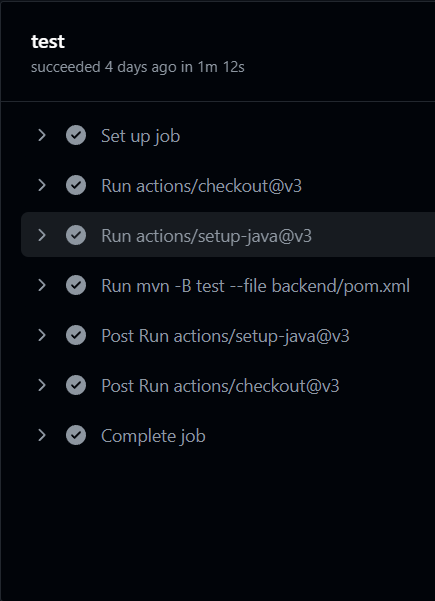
\includegraphics[width=0.3\textwidth]{tests.png}
        \label{fig:imagen3}
    \hfill
    }
    \subfloat[Creación de imagen Docker]{
        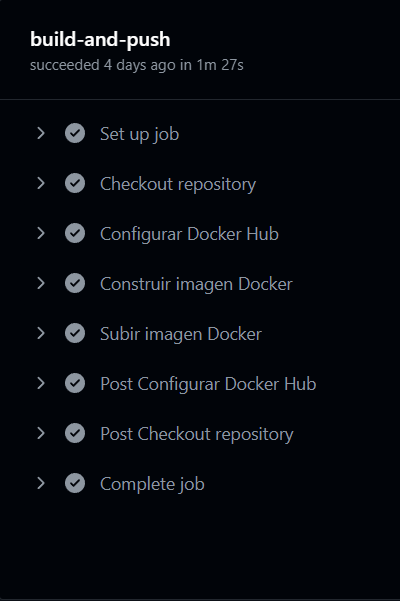
\includegraphics[width=0.3\textwidth]{dockerGIt.png}
        \label{fig:imagen2}
    }
    \hfill
    \subfloat[Conexión SSH con EC2]{
    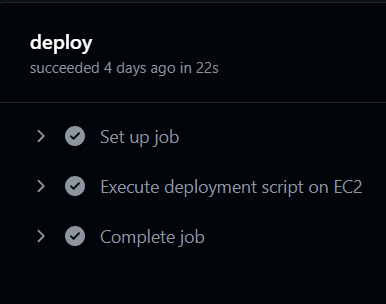
\includegraphics[width=0.4\textwidth]{ssh.png}
    \label{fig:imagen1}
    }
    \caption{Flujo de trabajos de GitHub}
    \label{fig:tripleta}
\end{figure}

\section{Estudio de Caso}
Dado que Enterprise Event Solutions es una aplicación diseñada para usuarios comunes, se ha llevado a cabo un estudio para recopilar opiniones y percepciones
 sobre la aplicación. En este estudio se incluyen preguntas tanto antes como después del uso de la aplicación por parte de los usuarios. Para la recolección de datos, 
 se utilizó Google Forms, y los resultados obtenidos se presentan en la sección de Apéndice.

\subsection{Participantes}
Debido a que la aplicaciones tiene diferentes tipos de usuarios he optado por seleccionar una serie de estos participantes para que interactuaran como organizadores,
como clientes o como administradores. En total se ha evaluado a 10 Participantes.
Cabe destacar que para la primera interacción con la aplicación se le ha requerido al Participante realizar una serie de pasos en la aplicación para 
valorar posteriormente la \textbf{usabilidad} y \textbf{accesibilidad} de esta.

\subsection{Valoración general}
En esta sección se desglosaran las preguntas y se expondrán los resultados.
\subsubsection*{Preguntas}
Para poder completar el estudio se han realizado las siguientes preguntas:
\begin{enumerate}
    \item Edad
    \item Uso habitual de dispositivos electrónicos
    \item ¿Sueles acudir a eventos de Empresas u Organizaciones?
    \item ¿Sueles leer los correos que te envían empresas promocionando eventos? 
    \item Como cliente ¿Cuál es tu opinión acerca de una aplicación que concentre la gestión de Eventos con la gestión de tus Entradas?
    \item ¿Darías uso a esta aplicación?
    \item Como Empresa ¿Cuál es tu opinión acerca de una aplicación que concentré la gestión tus Eventos con la gestión de la asistencia a estos?
    \item ¿Darías uso a esta aplicación?
    \item Después de haber probado la aplicación. ¿Con que asiduidad la usarías?
    \item ¿Cuál es tu opinión general sobre Enterprise Event Solutions?
\end{enumerate}
\subsubsection*{Resultados}
Los resultados del estudio de caso sobre la aplicación Enterprise Event Solutions son muy alentadores. La alta frecuencia de uso indicada por el \(80\%\)
de los usuarios sugiere que la aplicación cumple efectivamente con sus expectativas y necesidades. Además, la opinión general extremadamente positiva, con un \(100\%\) 
de los usuarios calificándola entre buena y excelente, refuerza la percepción de que Enterprise Event Solutions es una herramienta valiosa y bien recibida en su mercado objetivo. 
Estos resultados no solo reflejan la eficacia y utilidad de la aplicación, sino que también indican un alto potencial para su adopción y recomendación futura por parte de los usuarios 
satisfechos.

En el apéndice \ref{sec:apen1} se pueden ver los resultados desglosados de las preguntas realizadas a los participantes durante el Estudio.
\subsection{Desempeño}

Los usuarios detectaron un problema con la responsividad de la página en dispositivos móviles. Este problema
fue corregido tan pronto como se identificó el error.

\subsection{Diseño, Usabilidad y Accesibilidad}
En las primeras versiones de la aplicación, se observó que la interfaz gráfica carecía de ciertas facilidades para la navegación, como elementos
identificativos, códigos QR, flechas de navegación, spinners de carga y pantallas de error adecuadas. Además, el diseño dificultaba su uso, lo que llevó a una reestructuración completa de la página.

Es importante destacar que estos comentarios se recopilaron a lo largo del ciclo de vida del proyecto, y no únicamente en su etapa final.
Por lo tanto, considero que el contacto continuo con el usuario final es fundamental para lograr un producto refinado.

En rasgos generales los participantes consideran Enterprise Event Solutions una aplicación sencilla y fácil de entender.
